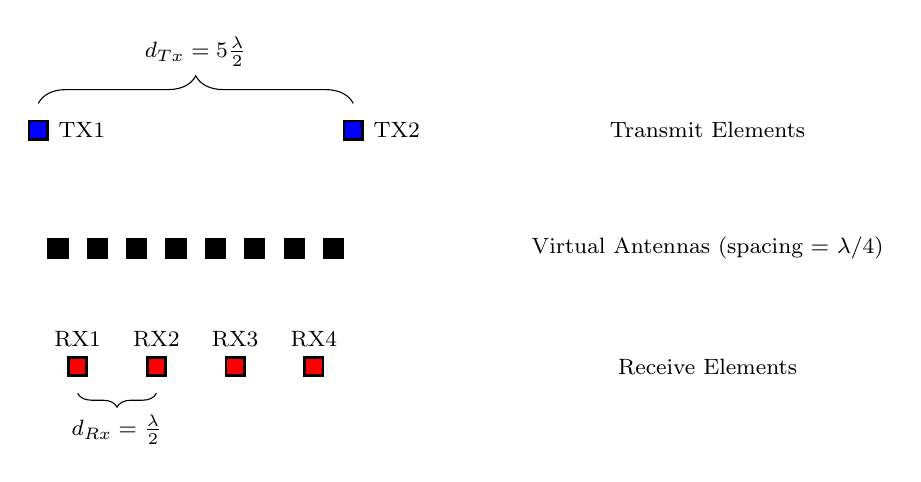
\begin{tikzpicture}
% Reference Grid
   \tikzstyle{tx} = [draw, shape=rectangle, minimum height=0.1cm, minimum width=0.1cm, node distance=0.0005cm and 0.0005cm, line width=1pt, fill = blue]
   \tikzstyle{rx} = [draw, shape=rectangle, minimum height=0.1cm, minimum width=0.1cm, node distance=0.0005cm and 0.0005cm, line width=1pt, fill = red]
   \tikzstyle{virt} = [draw, shape=rectangle, minimum height=0.1cm, minimum width=0.1cm, node distance=0.0005cm and 0.0005cm, line width=1pt, fill = black]
   
\node at (0.5,3) [tx,label =right: \footnotesize TX1](tx1){};
\node at (4.5,3) [tx,label =right: \footnotesize TX2] (tx2){}; 
\node at (1,0) [rx,,label =above: \footnotesize RX1] (rx1){}; 
\node at (2,0) [rx,label =above: \footnotesize RX2] (rx2){}; 
\node at (3,0) [rx,label =above: \footnotesize RX3] (rx3){}; 
\node at (4,0) [rx,label =above: \footnotesize RX4] (rx4){}; 
\path (tx1) -- (rx1) node[midway,virt] (virt1) {};
\path (tx1) -- (rx2) node[midway,virt] (virt2) {};
\path (tx1) -- (rx3) node[midway,virt] (virt3) {};
\path (tx1) -- (rx4) node[midway,virt] (virt4) {};
\path (tx2) -- (rx1) node[midway,virt] (virt5) {};
\path (tx2) -- (rx2) node[midway,virt] (virt6) {};
\path (tx2) -- (rx3) node[midway,virt] (virt7) {};
\path (tx2) -- (rx4) node[midway,virt] (virt8) {};

\draw [decorate,decoration={brace,amplitude=10pt,raise=4pt},yshift=0pt]
(0.5,3.2) -- (4.5,3.2) node [black,midway,yshift=0.8cm] {\footnotesize
	$d_{Tx} = 5\frac{\lambda}{2}$};
\draw [decorate,decoration={brace,mirror,amplitude=5pt,raise=4pt},yshift=0pt]
(1,-0.2) -- (2,-0.2) node [black,midway,yshift=-0.6cm] {\footnotesize
	$d_{Rx} = \frac{\lambda}{2}$};

\node at (9,3) [](n1) {\footnotesize Transmit Elements}; 
\node at (9,1.5) [](n1) {\footnotesize Virtual Antennas (spacing = $\lambda/4$)}; 
\node at (9,0) [](n1) {\footnotesize Receive Elements}; 
\end{tikzpicture}